\points{5b} \textbf{Implementing Inpainting through DDPM}

From the \texttt{inpaint.py} file, implement the masking function \texttt{get\_mask} by retaining only a central square of the image of side half of the image and 
the helper function \texttt{add\_forward\_tnoise}. Then update the noisy image $x_t$ to formulate the inpainting update in the \texttt{apply\_inpainting\_mask} function.

Run the inpainting experiment using the following command:
\begin{lstlisting}[language=bash]
    python run_sampling.py --dataset faces --experiment inpaint --image_path /path/to/image/to/inpaint
\end{lstlisting}

\textbf{Note: }For this problem we recommend using the faces dataset to see results visually. So before running the previous command one can first generate an image using ddim using the faces dataset Before running the previous command, you should first generate an image using DDIM with the faces dataset. Here's how:
\begin{lstlisting}[language=bash]
    python run_sampling.py --dataset faces --experiment ddim 
\end{lstlisting}

Below is the expected result from applying inpainting by specifying the DDIM image as the image to inpaint using the \texttt{--image\_path} argument:

\begin{figure}[H]
    \centering
    \begin{subfigure}[b]{0.25\textwidth}
        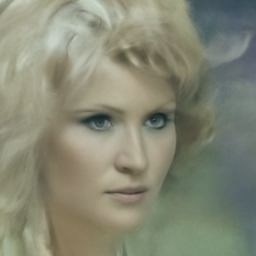
\includegraphics[width=\textwidth]{./figures/ddim_steps10_seed42_img_0}
        \caption{Original Image}
    \end{subfigure}
    \begin{subfigure}[b]{0.25\textwidth}
        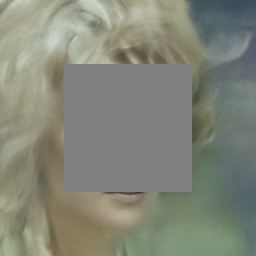
\includegraphics[width=\textwidth]{./figures/masked_ddim_steps10_seed42_img_0}
        \caption{Masked Image}
    \end{subfigure}
    \begin{subfigure}[b]{0.25\textwidth}
        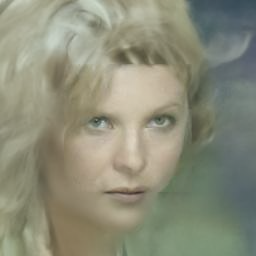
\includegraphics[width=\textwidth]{./figures/inpaint_steps1000_seed42_img_0}
        \caption{Inpainted Image}
    \end{subfigure}
\end{figure}